\chapter{Pixels, Polygons and Run-Length Encoding}\label{ch:masks}

\section{Introduction}\label{sec:masks-intro}
A segmentation model produces masks, the annotations are stored as polygons, and the competition's
scorer compares masks that are stored as compressed strings of text. In this chapter we study
these representations and the operations that connect them. Section~\ref{sec:masks-raster}
explains how a polygon is turned into a mask and why the details of that conversion matter so much
for thin objects. Section~\ref{sec:masks-rle} describes the run-length encoding used in the
submission file. Section~\ref{sec:masks-iou} defines the two standard measures of overlap between
masks, and Section~\ref{sec:masks-paint} describes how we turn a set of overlapping candidate masks
into the disjoint set that the rules require. These operations may look like routine plumbing, but
the first of them turned out to explain one of the largest improvements we made
(Section~\ref{sec:yolo-erosion}).

\section{From polygons to pixels}\label{sec:masks-raster}
A \keyterm{mask} is a binary image $M\in\{0,1\}^{H\times W}$, with $M_{ij}=1$ when pixel $(i,j)$
belongs to the object. An annotation, by contrast, is a polygon whose vertices have real-valued
coordinates. Converting a polygon into a mask is called \keyterm{rasterisation}, and it requires a
rule for the pixels that the boundary passes through. Is such a pixel inside the object if its
centre is inside the polygon? If any part of it is? If most of it is? Different software libraries
answer this question differently.

For a large, compact object the choice hardly matters, because the boundary pixels are a small
fraction of the total. A filament, however, is thin, so a large fraction of its pixels lie on or
near its boundary. Measured over the training annotations, the ratio of perimeter to area is about
$P/A=0.216$ per pixel. Suppose that two rasterisation rules place the boundary at positions that
differ by a distance $\delta$ all along its length. The area between the two boundaries is roughly
the perimeter times the offset, so the relative difference in area is
\begin{equation}
\frac{\Delta A}{A}\approx\frac{\delta\,P}{A}=0.216\,\delta .
\label{eq:masks-offset}
\end{equation}
A disagreement of only half a pixel therefore changes a filament's area by about 11\%.

\begin{figure}[t]
\centering
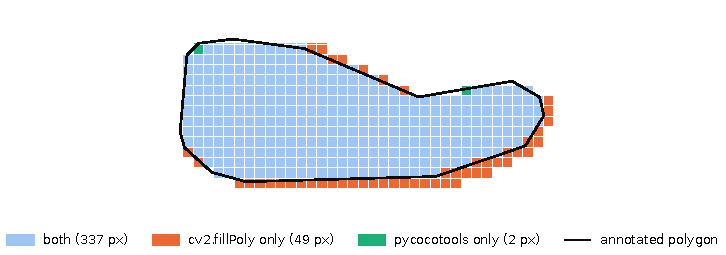
\includegraphics[width=\textwidth]{figures/fig_raster.pdf}
\caption{The same annotated polygon rasterised by two libraries. \texttt{cv2.fillPoly}, which
Ultralytics uses to build YOLO training targets, marks \RasterCv{} pixels; \texttt{pycocotools},
which the organisers' scorer uses, marks \RasterCoco{}. The IoU of the two masks is \RasterIoU{}.
\generatedby{book/make\_book\_figures.py:fig\_raster}}
\label{fig:masks-raster}
\end{figure}

Figure~\ref{fig:masks-raster} shows the effect on one real, thin filament. To measure it more
generally, we rasterised 400 randomly sampled training filaments with three common libraries (the
COCO tools \texttt{pycocotools}~\citep{coco}, OpenCV's \texttt{cv2}~\citep{bradski2000} and PIL)
and compared the results pair by pair (exp006):
\begin{center}\small
\begin{tabular}{@{}lcc@{}}
\toprule
pair of rasterisers & mean IoU & mean area relative to pycocotools \\
\midrule
pycocotools and cv2 & 0.874 & cv2 $+7.96\%$ \\
pycocotools and PIL & 0.915 & PIL $+5.71\%$ \\
cv2 and PIL & 0.897 & -- \\
\bottomrule
\end{tabular}
\end{center}
Two masks of the same polygon, both produced by standard software, agree with an IoU of less than
0.9. We will see in Chapter~\ref{ch:metric} that the metric requires an IoU above 0.5 before a
prediction counts at all, so a systematic error of this size uses up a substantial part of the
margin.

\subsection{Example: why the YOLO masks were too wide}\label{sec:masks-fat}
The competition's scorer rasterises the annotations with \texttt{pycocotools}. Ultralytics, the
library we used to train the YOLO models of Chapter~\ref{ch:yolo}, rasterises its training targets
with \texttt{cv2.fillPoly}. When we measured this end to end on our own pipeline, the YOLO training
targets agreed with the masks that the scorer uses with an IoU of 0.902, and they were
\textbf{10.8\% larger} on average, which is close to the value predicted by
Equation~\eqref{eq:masks-offset}. A model trained on these targets learns to draw every filament
slightly too wide, however well it is trained.

We noticed the effect before we understood it. In experiment exp005 we tried to \emph{grow} the
predicted masks, expecting that the model was cutting off thin barbs. Every amount of growth
lowered the score, whereas eroding every mask by one pixel raised it: validation PQ rose from
0.4169 to 0.4404, and the public score from 0.33 to 0.36, the largest single improvement of the
YOLO period. Section~\ref{sec:yolo-erosion} describes that experiment. The mismatch between the two
rasterisers explains about 95\% of the gain.

\subsection{Correcting in coordinates rather than pixels}\label{sec:masks-shrink}
Eroding a binary mask by one pixel is a coarse correction. It changed the area of the YOLO masks
from about 11\% too large to about 10\% too small. The ideal correction is half a pixel, and a
binary mask cannot be moved by half a pixel. To see why, consider the distance
transform~\citep{borgefors1986} of the mask, which gives each foreground pixel its distance to the
nearest background pixel. Every
boundary pixel is at distance 1, so thresholding the distance transform at 0.25, 0.5 or 0.75
returns the original mask unchanged.

Polygon coordinates have no such limitation. If we shrink each polygon inward by a fraction of a
pixel \emph{before} rasterising it, the correction is exact. We measured the effect of an inward
offset $\delta$ on 250 instances (exp006):
\begin{center}\small
\begin{tabular}{@{}lcccccc@{}}
\toprule
inward offset $\delta$ (px) & 0 & 0.25 & 0.35 & \textbf{0.50} & 0.65 & 1.00 \\
\midrule
IoU with the scorer's mask & 0.898 & 0.946 & 0.955 & \textbf{0.959} & 0.945 & 0.876 \\
area ratio & 1.112 & 1.039 & 1.019 & \textbf{0.986} & 0.954 & 0.876 \\
\bottomrule
\end{tabular}
\end{center}
An offset of half a pixel raises the agreement with the scorer from an IoU of 0.898 to 0.959.
Listing~\ref{lst:masks-shrink} shows the correction. It uses a polygon \emph{buffer}, which moves
every edge inward by the same perpendicular distance. Scaling the polygon towards its centroid
would be simpler, but it would move the ends of a long curved filament much further than its
middle. The code also guards against two failure modes that a naive buffer has on thin shapes. A
buffer can split a polygon at a narrow waist, which happened to 42 of the \AllFilaments{} training
filaments; in that case we keep the largest piece, so that one annotated filament never becomes two
training targets. A buffer can also erase a very thin shape altogether; in that case we keep the
original polygon.

\begin{lstlisting}[caption={Half-pixel inward offset for YOLO training targets. Simplified from \file{experiments/exp\_002\_yolo\_seg/src/prepare\_yolo.py:shrink}.},label=lst:masks-shrink]
from shapely.geometry import Polygon

def shrink(polygon, offset):
    """Offset a polygon inward by `offset` pixels, in coordinate space."""
    if offset <= 0 or len(polygon) < 3:
        return [polygon]
    shape = Polygon(polygon)
    if not shape.is_valid:
        shape = shape.buffer(0)          # repairs self-intersecting traces
    shrunk = shape.buffer(-offset)
    if shrunk.is_empty:                  # a very thin filament: keep the original
        return [polygon]
    geoms = [shrunk] if shrunk.geom_type == "Polygon" else list(shrunk.geoms)
    # One filament in, one filament out: if a narrow waist split it,
    # keep only the largest piece, never two instances where one was drawn.
    largest = max(geoms, key=lambda g: g.area)
    return [np.asarray(largest.exterior.coords, dtype=np.float64)]
\end{lstlisting}

The whole effect described in this section is invisible to a test that rasterises the ``ground
truth'' and the ``prediction'' with the same library, because such a test builds the answer into
its assumptions. We found the mismatch only by comparing the real training targets with the masks
that the real scorer computes. We return to this point in Chapter~\ref{ch:lessons}.

\section{Run-length encoding}\label{sec:masks-rle}
A $2048\times2048$ binary mask contains about four million pixels. Stored as one byte per pixel it
would occupy 4\,MB, but the competition's CSV file stores it in a few hundred bytes using the
\keyterm{run-length encoding} (RLE) of the COCO dataset~\citep{coco}. The idea is simple. We flatten the mask
into one long vector and record only the lengths of the alternating runs of zeros and ones.

COCO fixes two conventions. First, the flattening is \keyterm{column-major}: we read down the
first column, then down the second, and so on.\footnote{Column-major order is the convention of
Fortran and MATLAB, which is why NumPy~\citep{harris2020} calls arrays stored this way
``Fortran-ordered''.} Second, the first run always counts zeros, so a mask
whose first pixel is a one begins with a run of length zero. Figure~\ref{fig:masks-rle} works
through a $6\times6$ example.

\begin{figure}[t]
\centering
\begin{tikzpicture}[scale=0.42]
  \foreach \c/\r in {1/1,1/2,2/1,2/2,2/3,3/2,3/3,3/4,4/3,4/4} {
    \fill[vizblue!55] (\c,-\r) rectangle ++(1,-1);
  }
  \draw[step=1, gridline!80!black, line width=0.3pt] (0,0) grid (6,-6);
  \draw[inkprimary, line width=0.6pt] (0,0) rectangle (6,-6);
  \foreach \c in {0,...,5} \draw[->, vizorange, line width=0.6pt] (\c+0.5,0.25) -- (\c+0.5,-0.2);
  \node[note, anchor=south] at (3,0.4) {read each column top to bottom, left to right};
  \node[anchor=west, font=\ttfamily\scriptsize, text=inkprimary, align=left] at (7,-1.3)
    {0000000 11 0000 111 0000 111 0000 11 0000000};
  \node[anchor=west, note, align=left] at (7,-2.5) {runs: 7, 2, 4, 3, 4, 3, 4, 2, 7 \ \ (zeros first)};
  \node[anchor=west, note, align=left] at (7,-3.7) {differences from the run two back (from the fourth):\\ 7, 2, 4, 1, 0, 0, 0, $-$1, 3};
  \node[anchor=west, font=\ttfamily\small, text=inkprimary] at (7,-5.2) {counts = "7241000O3"};
\end{tikzpicture}
\caption{Run-length encoding of a $6\times6$ mask with 10 foreground pixels. Flattening the mask in
column-major order gives nine runs. COCO then stores each run from the fourth onwards as its
difference from the run two places earlier, writes each number in groups of 5 bits, and adds 48 to
every group so that it prints as an ASCII character. The string shown was produced by
\texttt{pycocotools}. \drawnin{book/chapters/ch03\_masks.tex}}
\label{fig:masks-rle}
\end{figure}

\subsection{The compressed string *}\label{sec:masks-rle-string}
A plain list of run lengths would still waste space on long runs, so COCO compresses it further.
Each run length, from the fourth onwards, is replaced by its \emph{difference} from the run length
two positions earlier. Consecutive columns of a filament tend to have similar runs, so these
differences are small. Each number is then split into groups of 5 bits, lowest bits first; a sixth
bit in each group marks whether another group follows; and 48 is added to the result so that it is
a printable character. In the example of Figure~\ref{fig:masks-rle}, the eighth run is 2 and the
sixth is 3, so the stored difference is $-1$. In two's complement arithmetic the lowest five bits
of $-1$ are 31, no further group is needed, and $31+48=79$ is the character \texttt{O}. The whole
mask becomes the nine characters \texttt{7241000O3}.

\subsection{Encoding and decoding in practice}\label{sec:masks-rle-code}
In practice we never write this encoder ourselves. Listing~\ref{lst:masks-rle} shows the two helper
functions through which every one of our submissions passes. The only subtle detail is the call to
\texttt{np.asfortranarray}. The \texttt{pycocotools} library expects the mask in column-major
memory order, and if it is given an ordinary row-major NumPy array it silently encodes the
transposed mask.

\begin{lstlisting}[caption={Encoding and decoding submission masks. From \file{shared/utils.py}.},label=lst:masks-rle]
from pycocotools import mask as mask_util

def encode_rle(binary_mask):
    """A binary (H, W) mask -> the COCO RLE `counts` string of the submission."""
    mask = np.asfortranarray(binary_mask.astype(np.uint8))
    return mask_util.encode(mask)["counts"].decode("utf-8")

def decode_rle(counts, size=(2048, 2048)):
    rle = {"size": list(size), "counts": counts.encode("utf-8")}
    return mask_util.decode(rle)
\end{lstlisting}

RLE is also the right format for storing masks between processing steps. On one occasion we cached
dense $2048\times2048$ masks for a parameter sweep; this took about 9\,GB per level of erosion, and
the process was killed for lack of memory. The same masks stored as RLE take a few kilobytes each.
The functions \texttt{pycocotools.mask.iou} and \texttt{pycocotools.mask.area} also operate
directly on RLE, so most measurements never need a dense mask at all.

\section{Comparing masks: IoU and Dice}\label{sec:masks-iou}
There are two standard ways to compare a predicted mask $A$ with an annotated mask $B$. The
\keyterm{intersection over union}, which ecologists know as the Jaccard index~\citep{jaccard1912},
is
\begin{equation}
\IoU(A,B)=\frac{|A\cap B|}{|A\cup B|},
\end{equation}
and the \keyterm{Dice coefficient}~\citep{dice1945} is
\begin{equation}
\mathrm{Dice}(A,B)=\frac{2|A\cap B|}{|A|+|B|}.
\end{equation}
Both are 1 for identical masks and 0 for disjoint ones, and in fact each can be computed from the
other. Writing $I=|A\cap B|$ and $U=|A\cup B|=|A|+|B|-I$, we have $\mathrm{Dice}=2I/(U+I)$, and
dividing the numerator and denominator by $U$ gives
\begin{equation}
\mathrm{Dice}=\frac{2\,\IoU}{1+\IoU},\qquad \IoU=\frac{\mathrm{Dice}}{2-\mathrm{Dice}}.
\label{eq:masks-dice-iou}
\end{equation}
Since $\IoU\le1$, Dice is never smaller than IoU. This is why the mean Dice of our final model
over overlapping pairs (\MeanDiceOverlap{}) looks better than its mean IoU (\MeanIoUOverlap{}),
although the two numbers describe the same masks. The leaderboard uses IoU, through Panoptic
Quality; the competition's rubric also asks for the distribution of Dice.

For thin objects both measures are very sensitive to small displacements. Consider a long filament
four pixels wide, and a copy of it shifted sideways by one pixel. Ignoring the ends, the
intersection is three pixels wide and the union five, so the IoU is $3/5=0.6$. With a shift of two
pixels the IoU falls to $2/6\approx0.33$, which is below the value of 0.5 that the metric requires
for a match. A disagreement of a few pixels about where a filament's edge lies can therefore decide
whether a prediction counts as a success or as two errors.

\section{From candidates to disjoint instances: painting}\label{sec:masks-paint}
Models do not naturally produce disjoint masks. A detector proposes candidates that may overlap,
while the scorer rejects any submission whose masks overlap. We resolve overlaps with a simple
procedure that we call \keyterm{painting}, close to the heuristic that \citet{pq} use to turn
instance predictions into a panoptic output, summarised in Algorithm~\ref{alg:masks-paint} and
Figure~\ref{fig:masks-paint}. We sort the candidates by their confidence scores, highest first.
Each candidate in turn keeps only those of its pixels that no higher-scoring candidate has already
claimed, and it is discarded if too few pixels remain.

\begin{algorithmblock}{Painting: turning scored candidates into disjoint masks\label{alg:masks-paint}}
\item \textbf{input:} candidates $(s_k, m_k)$, each a score and a binary mask; minimum area $a_{\min}$
\item sort the candidates so that $s_1\ge s_2\ge\cdots$;
\item $C\leftarrow$ empty mask (the pixels claimed so far); $\mathcal{S}\leftarrow\emptyset$;
\item \textbf{for} $k=1,2,\dots$ \textbf{do}
\item \Ind $r_k\leftarrow m_k\wedge\neg C$ \quad (the pixels of $m_k$ not yet claimed);
\item \Ind \textbf{if} $|r_k|\ge a_{\min}$ \textbf{then} add $(s_k, r_k)$ to $\mathcal{S}$ and set $C\leftarrow C\vee r_k$;
\item \textbf{return} $\mathcal{S}$
\end{algorithmblock}

\begin{figure}[t]
\centering
\begin{tikzpicture}[scale=0.62]
  \begin{scope}
    \fill[vizblue!45] (0,0) ellipse (1.6 and 0.55);
    \fill[vizorange!45, rotate around={35:(1.0,0.2)}] (1.0,0.2) ellipse (1.5 and 0.45);
    \draw[vizblue!80!black, line width=0.7pt] (0,0) ellipse (1.6 and 0.55);
    \draw[vizorange!80!black, line width=0.7pt, rotate around={35:(1.0,0.2)}] (1.0,0.2) ellipse (1.5 and 0.45);
    \node[note] at (0,-1.3) {two candidates overlap};
    \node[note, text=vizblue!80!black] at (-1.2,0.95) {score 0.93};
    \node[note, text=vizorange!80!black] at (2.4,1.35) {score 0.88};
  \end{scope}
  \draw[flow] (3.4,0) -- (4.6,0);
  \begin{scope}[xshift=7cm]
    \begin{scope}
      \clip (-3,-2) rectangle (3,2);
      \fill[vizorange!45, rotate around={35:(1.0,0.2)}] (1.0,0.2) ellipse (1.5 and 0.45);
      \fill[vizblue!45] (0,0) ellipse (1.6 and 0.55);
    \end{scope}
    \draw[vizblue!80!black, line width=0.7pt] (0,0) ellipse (1.6 and 0.55);
    \node[note] at (0,-1.3) {the higher score keeps the overlap;\\ the other keeps only unclaimed pixels};
  \end{scope}
\end{tikzpicture}
\caption{Painting resolves overlaps. Candidates are placed in order of decreasing score, and each
keeps only the pixels that no earlier candidate has claimed. \drawnin{book/chapters/ch03\_masks.tex}}
\label{fig:masks-paint}
\end{figure}

\begin{lstlisting}[caption={Overlap resolution by painting. From \file{shared/utils.py:paint\_panoptic}.},label=lst:masks-paint]
def paint_panoptic(candidates, min_area=150, image_size=(2048, 2048)):
    """Resolve overlapping (score, mask) candidates into a pixel-disjoint set."""
    ordered = sorted(candidates, key=lambda c: -c[0])
    claimed = np.zeros(image_size, dtype=np.uint8)
    kept = []
    for score, binary in ordered:
        remaining = (binary.astype(np.uint8) & (1 - claimed)).astype(np.uint8)
        area = int(remaining.sum())
        if area < min_area:
            continue
        claimed |= remaining
        kept.append((score, remaining, area))
    return kept
\end{lstlisting}

Painting has two properties that we will use later. First, a candidate can never take pixels from
a candidate with a higher score. Adding low-scoring candidates to the pool therefore cannot destroy
a match that already exists, which is why the recall experiments of Chapter~\ref{ch:recall} could
only ever cost us false positives and never lost true positives. Second, the minimum area is
applied \emph{after} the overlaps have been removed, so a candidate that loses most of its pixels
to a neighbour disappears altogether. The final model uses a minimum area of 100 pixels, and the
YOLO models used 300.

\section*{Exercises}
\begin{exercise}{The boundary approximation}
Derive Equation~\eqref{eq:masks-offset} for a rectangle of length $L$ and width $w$ that is shrunk
inward by $\delta$ on every side, and find the conditions under which the approximation is poor.
For a filament with $w=4$ pixels, what inward offset changes the area by 25\%?
\end{exercise}

\begin{exercise}{Encoding by hand}
Encode the transpose of the mask in Figure~\ref{fig:masks-rle} by hand, and check your string with
\texttt{pycocotools.mask.encode}. Then repeat the encoding without \texttt{np.asfortranarray}, and
explain the result.
\end{exercise}

\begin{exercise}{Dice and IoU}
Prove Equation~\eqref{eq:masks-dice-iou}, and show that $\mathrm{Dice}\ge\IoU$, with equality only
at 0 and 1. What value of Dice corresponds to the matching threshold $\IoU=0.5$?
\end{exercise}

\begin{exercise}{Painting order}
Write a test for \texttt{paint\_panoptic} that uses three overlapping random masks. Check that the
output is pixel-disjoint and that permuting the input does not change it. What happens when two
candidates have exactly the same score?
\end{exercise}

\begin{exercise}{A rasteriser audit}
Reproduce the first table of Section~\ref{sec:masks-raster} for 400 random training filaments, and
plot the ratio of the \texttt{cv2} area to the \texttt{pycocotools} area against each filament's
ratio of perimeter to area. Does the slope agree with Equation~\eqref{eq:masks-offset}?
\end{exercise}
